\documentclass[12pt]{exam}

% essential packages
\usepackage{fullpage} % margin formatting
\usepackage{enumitem} % configure enumerate and itemize
\usepackage{amsmath, amsfonts, amssymb, mathtools} % math symbols
\usepackage{xcolor, colortbl} % colors, including in tables
\usepackage{makecell} % thicker \Xhline in table
\usepackage{graphicx} % images, resizing

% sometimes needed packages
\usepackage{hyperref} % hyperlinks
% \hypersetup{colorlinks=true, urlcolor=blue}
% \usepackage{logicproof} % natural deduction
% \usepackage{tikz} % drawing graphs
% \usetikzlibrary{positioning}
% \usepackage{multicol}
% \usepackage{algpseudocode} % pseudocode

% paragraph formatting
\setlength{\parskip}{6pt}
\setlength{\parindent}{0cm}

% newline after Solution:
\renewcommand{\solutiontitle}{\noindent\textbf{Solution:}\par\noindent}

% less space before itemize/enumerate
\setlist{topsep=0pt}

% creates \filcl to grey out cells for groupwork grading
\newcommand{\filcl}{\cellcolor{gray!25}}

% creates \probnum to get the problem number
\newcounter{probnumcount}
\setcounter{probnumcount}{1}
\newcommand{\probnum}{\arabic{probnumcount}. \addtocounter{probnumcount}{1}}

% use roman numerals by default
\setlist[enumerate]{label={(\roman*)}}

% creates custom list environments for grading guidelines, question parts
\newlist{guidelines}{itemize}{1}
\setlist[guidelines]{label={}, left=0pt .. \parindent, nosep}
\newlist{gwguidelines}{enumerate}{1}
\setlist[gwguidelines]{label={(\roman*)}, nosep}
\newlist{qparts}{enumerate}{2}
\setlist[qparts]{label={(\alph*)}}
\newlist{qsubparts}{enumerate}{2}
\setlist[qsubparts]{label={(\roman*)}}
\newlist{stmts}{enumerate}{1}
\setlist[stmts]{label={(\roman*)}, nosep}
\newlist{pflist}{itemize}{4}
\setlist[pflist]{label={$\bullet$}, nosep}
\newlist{enumpflist}{enumerate}{4}
\setlist[enumpflist]{label={(\arabic*)}, nosep}

\printanswers

\newcommand{\prevhwnum}{4}
\newcommand{\hwnum}{5}

\begin{document}
\section*{Individual Portion}

\subsection*{\probnum Easy as 3, 18, 93 [16 points]}

Let $P(n)$ be the statement that $3 + 3 \cdot 5 + 3 \cdot 5^2 + ... + 3 \cdot 5^n = \frac{3 (5^{n+1} - 1)}{4}$. In this problem, we will prove using weak induction that $P(n)$ is true whenever $n$ is a non-negative integer.
\begin{parts}
	\item What is the statement $P(0)$? Complete the base case by showing that $P(0)$ is true.
	\item In the base case we prove $P(0)$; what do you need to prove in the inductive step?
	\item What is the inductive hypothesis for your proof?
	\item Complete the inductive step, indicating where you used the inductive hypothesis.

	\textit{Reminder:} You should prove this equation using a chain of equalities, starting on one side and transforming it into the other side.  You should \textbf{not} start with the equation you want to prove and transform both sides to be equal.
	\item Explain why this proof shows $P(n)$ is true for all non-negative integers $n$.
\end{parts}

\begin{solution}
	a) $P(0)$ is the statement that $3 + 3 \cdot 5 + 3 \cdot 5^2 + ... + 3 \cdot 5^0 = \frac{3 (5^{0+1} - 1)}{4}$.\\
	Base case: $P(0)$, LHS$=3 \cdot 5^0=3$, RHS$=\frac{3(5-1)}{4}=\frac{3(4)}{4}=3$\\
	Since LHS=RHS, the base case holds.\\
	\\ b) Let $k$ be arbitary $ k \in \mathbb{Z}^+$ , want to show $P(k) \rightarrow P(k+1)$\\
	c) The inductive hypothesis is assume that $P(k)$ is true.\\
	d)\\
	\begin{tabular}{ll}
		Assume $P(k)$.                                                       \\
		LHS:                                                                 \\
		$=3 + 3 \cdot 5 + 3 \cdot 5^2 + ... +3 \cdot 5^{k}+ 3 \cdot 5^{k+1}$ \\
		$=\frac{3 (5^{k+1} - 1)}{4}+3 \cdot 5^{k+1}$ & I.H.                  \\
		$=\frac{3(5^{k+1}-1)+ 3 \cdot 4 \cdot 5^{k+1}}{4}$                   \\
		$=\frac{3(5\cdot 5^{k+1}-1)}{4}$                                     \\
		$=\frac{3(5^{k+2}-1)}{4}$                                            \\
		RHS:                                                                 \\
		$=\frac{3(5^{k+2}-1)}{4}$                                            \\
		Since LHS$=$RHS, $P(k+1)$ holds.
	\end{tabular}
	\\e) This proof shows $P(n)$ is true by proof by weak induction.\\
	This is because since the base case holds and the inductive step holds, $P(n)$ is true for all non-negative integers $n$.
\end{solution}


\subsection*{\probnum Inequality Induction [16 points]}
Let $P(n)$ be the following inequality: \(2^n > n\). Use weak induction to prove that $P(n)$ is true for all positive integers.
\begin{parts}
	\item What is the statement $P(1)$? Complete the base case by showing that $P(1)$ is true.
	\item What do you want to show in the inductive step?
	\item What is the inductive hypothesis for your proof?
	\item Complete the inductive step, indicating where you used the inductive hypothesis.
	\item Conclude your proof by explaining why the above shows $P(n)$ is true for all positive integers $n$.
\end{parts}
\begin{solution}
	a) $P(1)$ is the statement that $2^1>1$.\\
	Base case: $P(1)$, LHS$=2$, RHS$=1$. Since LHS$>$RHS, the base case holds.\\
	b) Want to show $P(k) \rightarrow P(k+1)$\\
	c) The inductive hypothesis is assume that $P(k)$ is true.\\
	d)\\
	\begin{tabular}{ll}
		Assume $P(k)$. \\
		LHS:           \\
		$=2^{k+1}$     \\
		$=2\cdot 2^k$  \\
		$=k+k$ & I.H.  \\
		RHS:           \\
		$=k+1$         \\
		Since $k>1, k+k>k+1$, LHS$>$RHS, $P(k+1)$ holds.
	\end{tabular}
	\\e) This proof shows $P(n)$ is true by proof by weak induction.\\
	This is because since the base case holds and the inductive step holds, $P(n)$ is true for all positive integers $n$.
\end{solution}

\subsection*{\probnum Divisible Induction [16 points]}
Prove by induction that 5 divides $3^{4n}+4$ whenever $n$ is a positive integer

\begin{solution}
	Proof:\\
	Proof by weak induction.\\
	\begin{tabular}{ll}
		Let $P(n)$ be the statement $\forall n, 5\mid 3^{4n}+4, n\in \mathbb{Z}^+$                         \\
		In other words, $\forall n, \exists m$ such that $3^{4n}+4=5m, m\in \mathbb{Z}, n\in \mathbb{Z}^+$ \\
		Want to show: $P(k)\rightarrow P(k+1)$                                                             \\
		Inductive step:                                                                                    \\
		Assume $P(k)$.                                                                                     \\
		By I.H. $3^{4k}=5m-4, m\in \mathbb{Z}$ for some $m$                                                \\
		LHS:                                                                                               \\
		$3^{4(k+1)}+4$                                                                                     \\
		$=3^{4k+4}+4$                                                                                      \\
		$=3^{4k}\cdot 3^4+4$                                                                               \\
		$=(5m-4)\cdot 3^4+4$                          & I.H.                                               \\
		$=81\cdot 5m-4\cdot 3^4+4$                                                                         \\
		$=3^4\cdot 5m -4\cdot (3^4-1)$                                                                     \\
		$=3^4\cdot 5m -4\cdot 80$                                                                          \\
		$=5(3^4m-64)$                                                                                      \\
		Let  $j=3^4m-64$                                                                                   \\
		$=5j$                                                                                              \\
		Since $j$ is an integer, $P(k+1)$ holds.      & definition of divide                               \\


		Base case:                                                                                         \\
		$P(1)=3^4+4=85$                                                                                    \\
		Let $j$ be a number, $5j=85, j=17$                                                                 \\
		Since $j$ is an integer, the base case holds. & definition of divide                               \\

		By weak induction, $P(n)$ is true for all positive integers $n$.
	\end{tabular}
\end{solution}


\subsection*{\probnum Please Pretend Postage Pun Present [12 points]}
Let $P(n)$ be the predicate ``$n$ cents can be formed using $3$ and $7$ cent stamps."
\begin{qparts}
	\item Find the smallest $c\in \mathbb N$ so that $\forall n\ge c,\ P(n)$.
	\item Prove by induction that $\forall n\ge c,\ P(n)$. Use the minimum number of base cases needed.
\end{qparts}

\begin{solution}
	a) Consider $c=10=3+7$ whereas $c=11$ does not work. Thus, the smallest $c\in \mathbb N$ so that $\forall n\ge c,\ P(n)$ is $c=12$.\\
	b)\\
	Proof:                                                                                  \\
	Proof by strong induction.                                                              \\
	Let $P(n)$ be the statement that $n$ cents can be formed using $3$ and $7$ cent stamps. \\
	Let $k\in \mathbb{Z}^+, k\ge 14, k$ be arbitary                                         \\
	\begin{tabular}{ll}
		Inductive step:                                          \\
		Assume $P(j), \forall j(12\le j\le k-1)$                 \\
		Want to show: $P(j)\rightarrow P(j+3)$                   \\
		$j=3a+7b$ for some $a,b\in \mathbb{Z}^+$, $a+b=j$ & I.H. \\
		Then $j+3=3(a+1)+7b$                                     \\
		Since $a+1\in \mathbb{Z}^+$, $P(j+3)$ holds.             \\

		Base case:                                               \\
		$P(12)$: $12=3\cdot 4$                                   \\
		$P(13)$: $13=3\cdot 2+7$                                 \\
		$P(14)$: $14=7\cdot 2$                                   \\
	\end{tabular}
	\\Thus, by strong induction, $P(n)$ is true for all positive integers $n\ge 12$.
\end{solution}


\subsection*{\probnum Inductive Delights [14 points]}
Assume that a chocolate bar consists of $n\geq 1$ squares arranged in a rectangular pattern. Any rectangular piece of the bar including the entire bar can be broken along a vertical or a horizontal line separating the squares. Assuming you can only break the bar along one axis at a time, determine how many breaks you must successively make to break the bar into $n$ separate squares. Use \textbf{strong induction} to prove your answer.

\pagebreak
\begin{solution}
	Proof: \\
	Proof by strong induction. \\
	Let $P(n)$ be the statement that $n-1$ breaks are needed to break the bar into $n$ separate squares. \\
	Let $k\in \mathbb{Z}^+, k\ge 2, k$ be arbitary \\
	Inductive step:                                                                  \\
	Assume $P(j), \forall j(1\le j\le k-1)$                                          \\
	Want to show: $P(k)$                                                             \\
	Take a chocolate bar with $k$ squares.                                           \\
	Break the bar into two pieces.                                                   \\
	Let $i\ge 1$ be the number of squares in the first piece,
	$k-i\le k-1$ be the second piece.                                                \\

	Since breaking chocolate into two separate pieces will always be the first step, \\
	\begin{tabular}{ll}
		$P(k)=P(i)+P(k-i)+1=j-1$     \\
		LHS:                         \\
		$=i-1+k-i-1+1$ & I.H.        \\
		$=k-1$                       \\
		RHS:                         \\
		$P(k)=k-1$                   \\
		Since LHS=RHS, $P(k)$ holds. \\
		Base case:                   \\
		$P(1)=1-1=0$                 \\
	\end{tabular}
	\\	Thus, by strong induction, $P(n)$ is true for all positive integers $n$.

\end{solution}


\subsection*{\probnum A Mess of Messages [12 points]}
We are sending messages made up of the characters ``a'', ``b'', and ``c''. An ``a'' takes 1 microsecond to send, and a ``b'' or ``c'' takes 2 microseconds to send. Let $M(n)$ denote the number of distinct messages we can send using exactly $n$ microseconds (in particular, the message cannot be sent in fewer than $n$ microseconds), for $n \ge 0$.

\begin{qparts}
	\item Give a recurrence relation for $M(n).$
	\item Give the initial conditions for your recurrence. Include only the minimum necessary conditions.
\end{qparts}

% template to phrase the a)
% If the lastpastrydecoratedwas acookie, thentherearean−2 possibleways to
% decorate. If the lastpastrydecoratedwasacupcake, therearean−3ways. If the
% lastpastrydecoratedwasapie, therearean−3ways. Therefore,ourrecurrenceis
% an=an−2+an−3+an−3=an−2+2an−3.
\begin{solution}
	a) Walking Backwards:\\
	If the last character is ``a'', then there are $M(n-1)$ possible ways to send the message.\\
	If the last character is ``b'' or ``c'', then there are $M(n-2)$ possible ways to send the message.\\
	Therefore, the recurrence relation is
	$M(n)=M(n-1)+M(n-2)+M(n-2)$
	$=M(n-1)+2M(n-2)$\\
	b) There is one message that can be sent in 0 microseconds, and that is the empty message.\\
	There are two messages that can be sent in 1 microsecond, and that is the message ``a'' and the empty message.\\
	$M(0)=1, M(1)=2$

\end{solution}

\subsection*{\probnum Carrot the Cat [14 points]}
Carrot the cat likes taking naps in one of four locations: the rug, the bed, the ledge, and the sink. Carrot has the following conditions:
\begin{itemize}
	\item He will not sleep in the sink twice in a row
	\item He will sleep on the ledge only if he slept on the rug the previous time
\end{itemize}
Let $L(n)$ be the number of possible sequences of locations for $n$ naps, where $n \ge 0.$

\begin{qparts}
	\item Give a recurrence relation for $L(n).$
	\item Give the initial conditions for your recurrence. Include only the minimum necessary conditions.
\end{qparts}

\begin{solution}
	a) Walking Backwards:\\
	Let cases be the last location Carrot slept in $n$ naps.\\
	Case 1: Rug\\
	If the last location is the rug, then there are $L(n-1)$ possible sequences.\\
	Case 2: Bed\\
	If the last location is the bed, then there are $L(n-1)$ possible sequences.\\
	Case 3: Ledge\\
	Since Carrot will sleep on the ledge only if he slept on the rug the previous time, then there are $L(n-2)$ possible sequences.\\
	Case 4: Sink\\
	Since Carrot will not sleep in the sink twice in a row, then there are $L(n-3)$ possible sequences.\\
	Adding all the cases, the recurrence relation is $L(n)=L(n-1)+L(n-1)+L(n-2)+L(n-3)=2L(n-1)+L(n-2)+L(n-3)$\\
	b) If Carrot does not take naps, there are zero locations.\\
	There are 3 locations that can be slept in 1 nap, i.e. rug, bed, or the sink.\\
	For the 2 naps, Carrot has 9 possible locations to sleep.\\
	$L(0)=1, L(1)=3, L(2)=9$

\end{solution}

\pagebreak
\setcounter{probnumcount}{1}
\section*{Groupwork \hwnum{} Problems}

\subsection*{\probnum Plane Cutting [12 points]}
If $n$ lines are drawn on a plane, no two lines are parallel, and all pairs of lines intersect at different points, how many sections do they separate the plane into? Assume that no more than two lines intersect at any one point.  Prove your result using weak induction. Don't include unneeded base cases.

\begin{solution}
	\begin{tabular}{ll}
		Proof:                                                                                       \\
		Proof by weak induction.                                                                     \\
		Let $P(n)$ be the statement that $n$ lines drawn on a plane separate the plane               \\
		into $\frac{n(n+1)}{2}+1$ sections.                                                          \\
		Let $k\in \mathbb{Z}^+, k\ge 1, k$ be arbitary                                               \\
		Inductive step:                                                                              \\
		Assume $P(k)$.                                                                               \\
		Want to show: $P(k+1)$                                                                       \\
		Take a plane with $k$ lines.                                                                 \\
		Add a new line.                                                                              \\
		This new line intersects the $k$ lines at $k$ different points.                              \\
		This new line separates the plane into $k+1$ new sections.                                   \\
		Thus, the total number of sections is:                                                       \\
		$\frac{k(k+1)}{2}+1+k+1=\frac{k^2+k+2k+2}{2}+1=\frac{k^2+3k+2}{2}+1=\frac{(k+1)(k+2)}{2}+1$. \\
		Since $P(k+1)$ holds, $P(n)$ is true for all positive integers $n$.                          \\
		Base case:                                                                                   \\
		LHS:                                                                                         \\
		$P(1)=\frac{1(1+1)}{2}+1=2$                                                                  \\
		RHS:                                                                                         \\
		$P(1)=P(0)+1=1+1=2$                                                                          \\
	\end{tabular}
	\\Thus, by weak induction, $P(n)$ is true for all positive integers $n$.
\end{solution}

\subsection*{\probnum Splitting Stones [18 points]}
In front of you sits a pile of $n$ stones.  You split the pile into two smaller piles, count the number of stones in the smaller pile, $j$, and write down the number $2^j$. Then, for each of the two piles, you split them and write down their versions of $2^j$.  You repeat this process, splitting piles and writing down exponentials until all piles have only 1 stone in them.  Finally, you multiply together all the numbers you wrote down.

For example, if we start with 8 stones, one possible way these piles could be split is as follows:

\begin{center}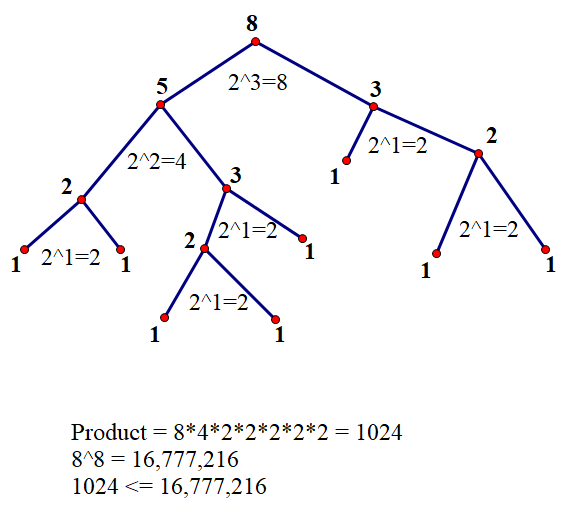
\includegraphics[scale=.75]{induction.png}\end{center}

Prove using strong induction that no matter how you split the piles, the overall product you get is less than or equal to $n^ n$.

\textbf{Hint:} When there is only one stone, you cannot split the pile, and the process stops.

\begin{solution}

	\begin{tabular}{ll}
		Proof:                                                                                   \\
		Proof by strong induction.                                                               \\
		Let $P(n)$ be the statement that the overall product is less than or equal to $n^n$.     \\
		Let $k\in \mathbb{Z}^+, k\ge 1, k$ be arbitary                                           \\
		Inductive step:                                                                          \\
		Assume $P(j), \forall j(1\le j\le k-1)$                                                  \\
		Want to show: $P(k)$                                                                     \\
		Take a pile of $k$ stones.                                                               \\
		Split the pile into two smaller piles.                                                   \\
		Let $i$ be the number of stones in the smaller pile.                                     \\
		Since $i\le k-1$, by I.H., the overall product of the smaller pile is $\le (k-1)^{k-1}$. \\
		The overall product of the larger pile is $\le (k-i)^{k-i}$.                             \\
		The overall product of the pile of $k$ stones is $\le i^{i}\cdot (k-i)^{k-i}$.           \\
		Since $i\le k-1$, $i^{i}\le (k-1)^{k-1}$.                                                \\
		Thus, the overall product of the pile of $k$ stones is:                                  \\
		$\le (k-1)^{k-1}\cdot (k-1)^{k-1}=(k-1)^{k-1}\cdot (k-1)^{k-1}=(k-1)^{k}$.               \\
		Since $P(k)$ holds, $P(n)$ is true for all positive integers $n$.                        \\
		Base case:                                                                               \\
		$P(1)=1^1=1$                                                                             \\
		Thus, by strong induction, $P(n)$ is true for all positive integers $n$.
	\end{tabular}
\end{solution}
\end{document}
